\chapter{Аналитический раздел}

\section{Анализ предметной области}
С увеличением числа сотрудников компании часто возникают проблемы внутренней коммуникации сотрудников, получения информации о коллегах и автоматизации процессов рекрутмента~\cite{intranet_avito}. Для решения этих задач существуют внутренние порталы для сотрудников. Обычно они представляют функционал, схожий с соцсетями: отображение профилей пользователей, и др. 

В основном, внутренние порталы для сотрудников представляют собой закрытые решения~\cite{глухих2005глухих}, которые разрабатываются в рамках одной компании~\cite{rivelty}, и не распространяются во внешний мир вследствии политики конфиденциальности~\cite{klee2000importance}. 



\section{Сравнение с аналогичными решениями}
В данной части проводится сравнение предлагаемого решения с аналогами~---~наиболее активно используемыми и разрабатываемыми известными внутренними порталами для сотрудников~\cite{rivelty}.

\paragraph{Критерии сравнения} \mbox{}

В качестве критериев сравнения решений были выбраны основные элементы функционала:

\begin{enumerate}
	\item возможность просматривать профили пользователей;
	\item хранение информации об иерархии сотрудников;
	\item возможность хранить информацию о команде сотрудника;
	\item отсутствие платы за использование;
	\item открытость решения для использования.
\end{enumerate}


\paragraph{Сравнение} \mbox{}

В таблице \ref{table:anal_compare} приведено сравнение решений для внутреннего портала для сотрудников организации.

\begin{table}[h]
  \caption{\label{table:anal_compare} Сравнение существующих решений с предложенным}
  \begin{center}
    \begin{tabular}{|l|l|l|l|l|l|}
      \hline
      Решение              & 1 & 2 & 3 & 4 & 5 \\ \hline
      Интранет VK~\cite{intranet_vk}          & $+$ & $+$ & $-$ & $+$ & $-$ \\ \hline
      Avito People~\cite{intranet_avito}         & $+$ & $+$ & $+$ & $+$ & $-$ \\ \hline
      Битрикс24~\cite{bitrix24}           & $+$ & $+$ & $-$ & $-$ & $+$ \\ \hline
      Предлагаемое решение & $+$ & $+$ & $+$ & $+$ & $+$ \\ \hline
    \end{tabular}
  \end{center}
\end{table}

\section{Формализация задачи}
Решение должно представлять собой портал, в котором будет производиться регистрация сотрудника менеджером по персоналу. Сотрудник сможет просматривать профили других сотрудников, производить поиск по организации.

Каждый сотрудник состоит в некоторой иерархии: у него есть руководитель и подразделение, в котором он находится. Кроме того, роль сотрудника может не совпадать с его положением в этой иерархии~\cite{intranet_avito}. Например, по документам он может находиться в департаменте разработки, а фактически находиться в команде какого-либо проекта. Решение должно учитывать эту особенность.

Сотрудник может редактировать основные данные профиля: фотографию, описание профиля, информацию об отпуске, при этом такую информацию, как имя, должность и положение в иерархии компании может изменять только рекрутер.


\paragraph{Формализация сценариев использования} \mbox{}

В рамках решения должно существовать три вида пользователей:

\begin{enumerate}
	\item Сотрудник~---~сотрудник предприятия. Имеет базовые возможности по изменению части информации профиля, поиску среди пользователей системы.
	\item Рекрутер~---~менеджер по персоналу. Может создавать профили сотрудников, удалять их, изменять базовую информацию, такую как имя, должность.
	\item Администратор~---~главная роль в системе. Может делать то же, что может рекрутер. Кроме того, может редактировать базовую структуру организации, и управлять другими администраторами.
\end{enumerate}

На рис.~\ref{img:use-case} изображена диаграмма сценариев использования предлагаемого решения.

\begin{figure}[h!]
\centering
    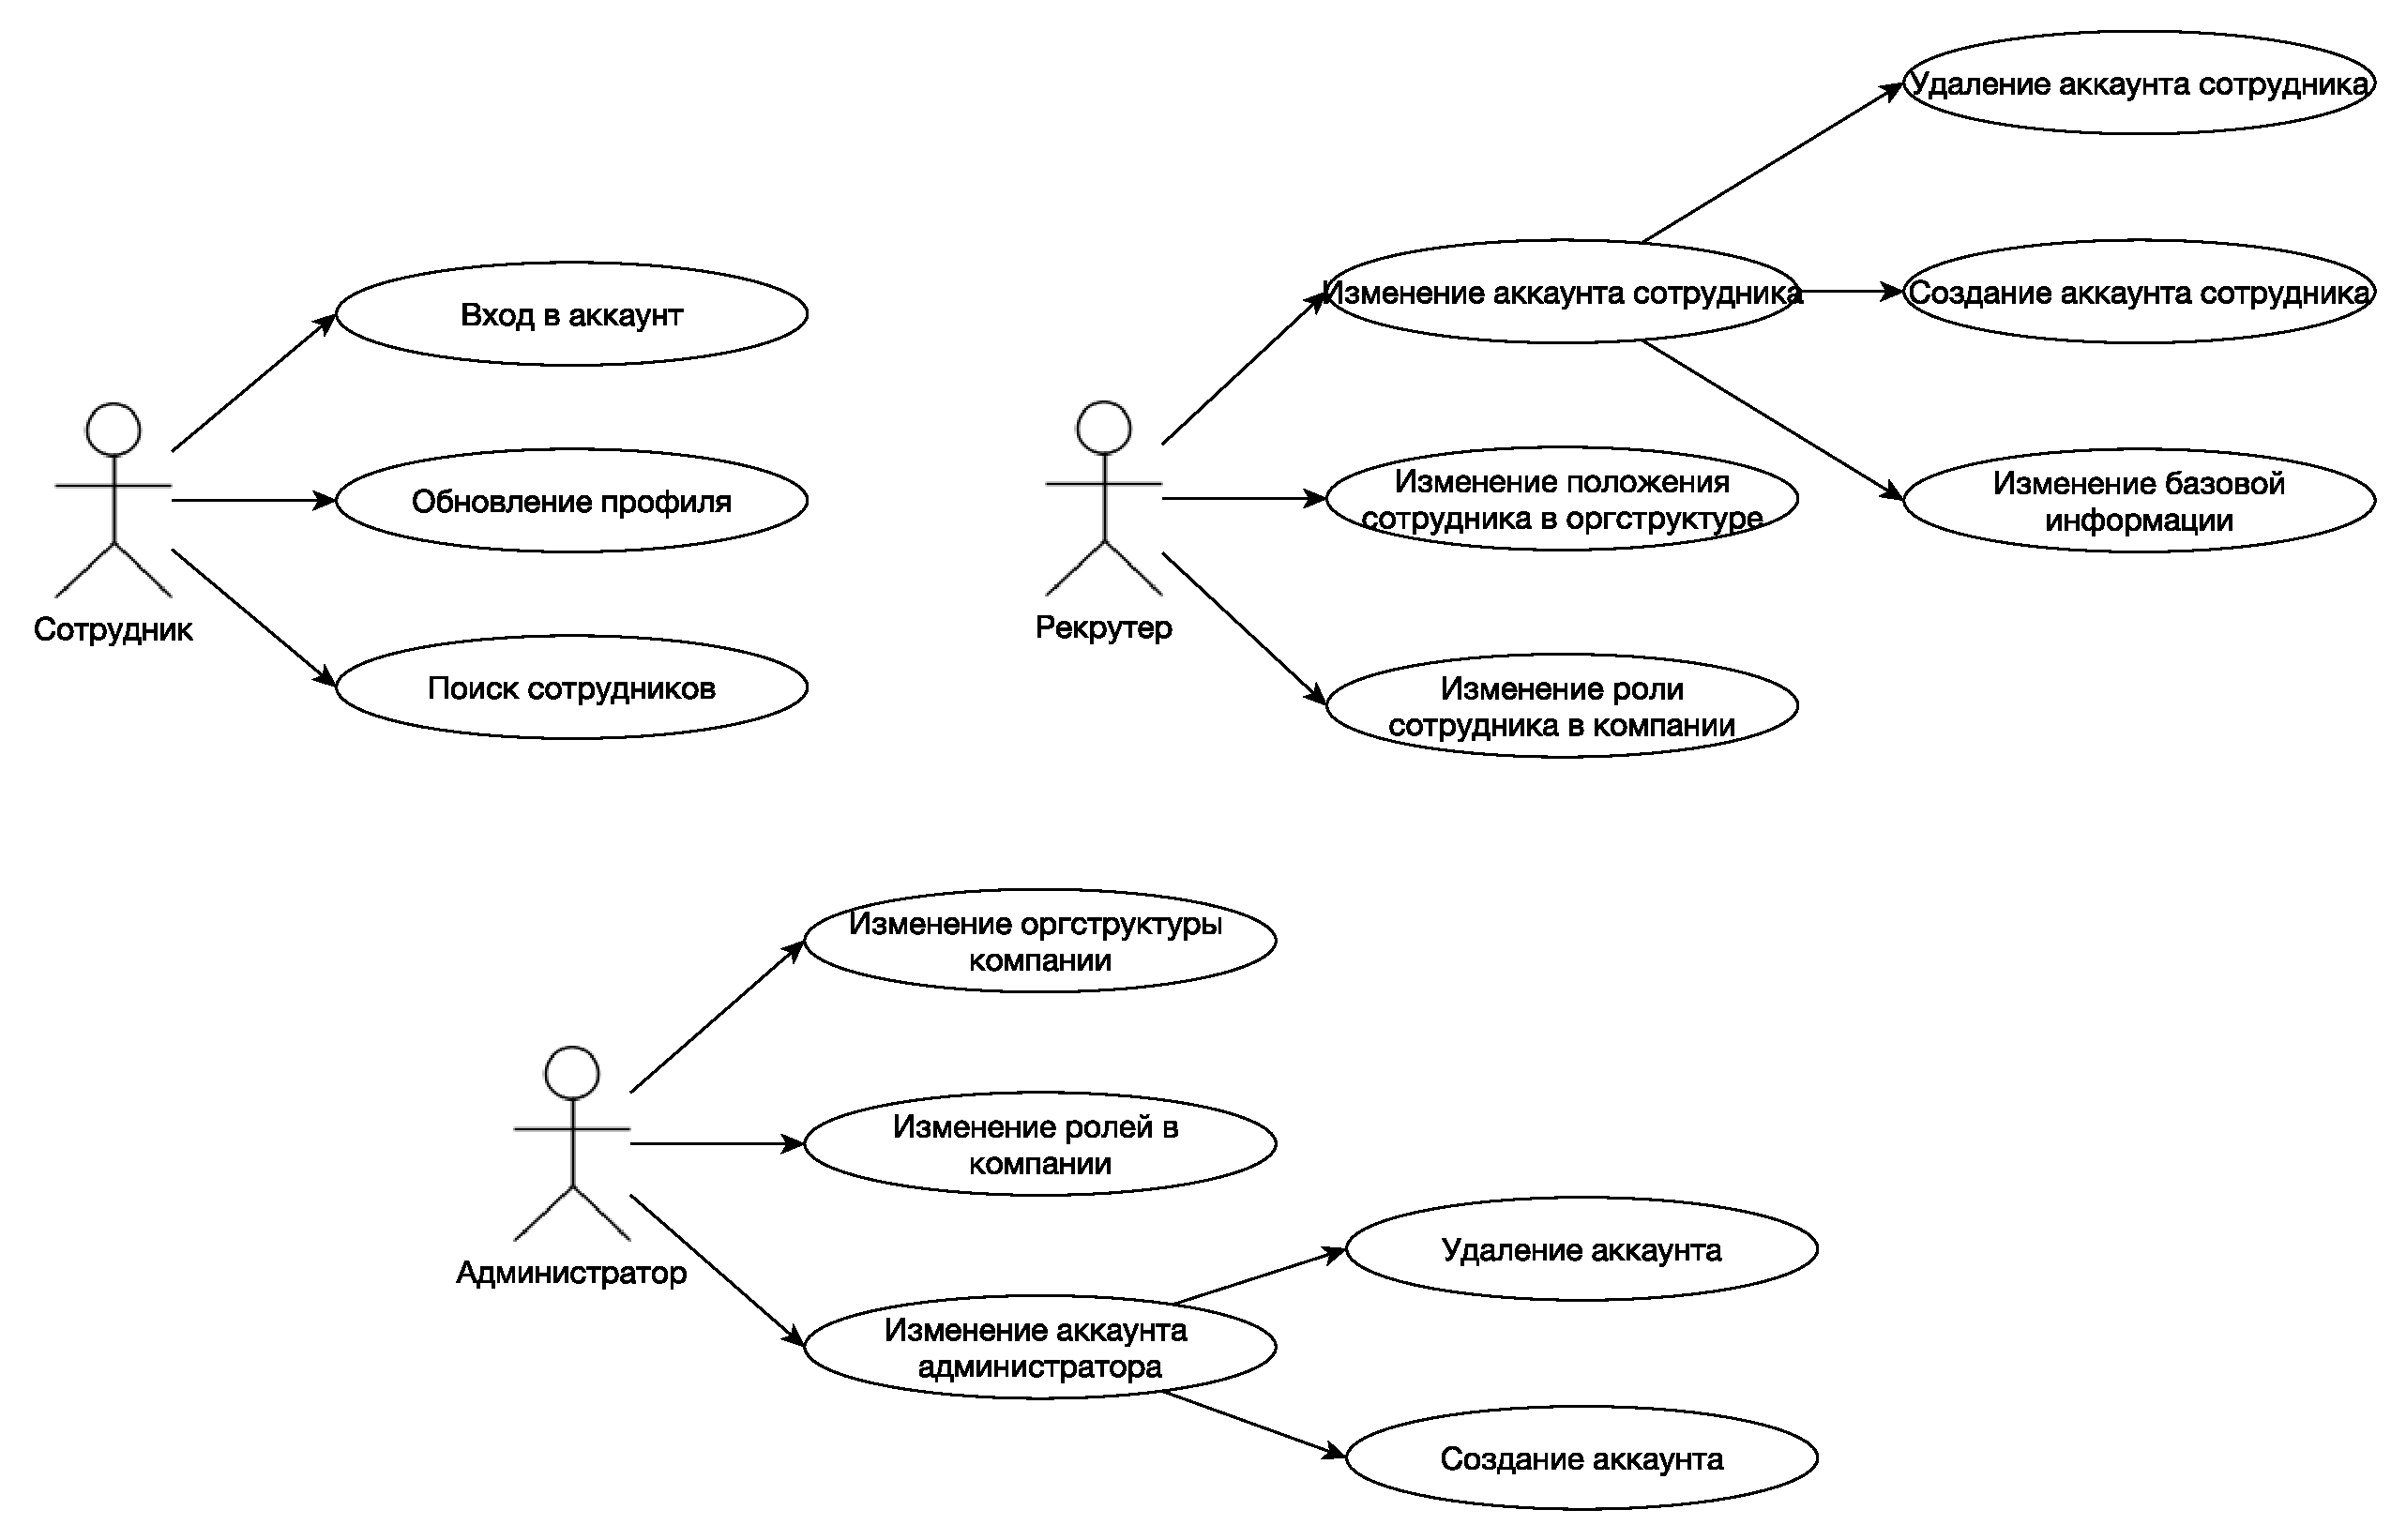
\includegraphics[width=0.9\linewidth]{assets/use-case.pdf}
    \caption{Диаграмма сценариев использования (начало)}
    \label{img:use-case}	
\end{figure}

%\begin{figure}[h!]
%\centering
%    \includegraphics[width=0.8\linewidth]{assets/use-case1.pdf}
%    \caption{Диаграмма сценариев использования (конец)}
%    \label{img:use-case1}	
%\end{figure}


\paragraph{Формализация данных} \mbox{}

Основные сущности, которые должны содержаться в проектируемой базе данных:

\begin{itemize}
	\item сотрудник;
	\item команда~---~фактическая команда, в которой работает сотрудник;
	\item подписка;
	\item отпуск;
	\item отдел~---~официальный департамент, в который трудоустроен сотрудник.
\end{itemize}

На рис.~\ref{img:chen} изображена ER-диаграмма сущностей проектируемой базы данных в нотации Чена.

\newpage

\begin{figure}[h!]
\centering
    \includegraphics[width=0.9\linewidth]{assets/chen.pdf}
    \caption{ER-диаграмма сущностей в нотации Чена}
    \label{img:chen}	
\end{figure}


\section{Виды СУБД по модели данных}

База данных представляет собой набор связанных данных некоторой предметной области, поэтому для ее организации важно определиться с моделью данных. Модель данных представляет собой логическую структуру данных, хранящихся в базе данных~\cite{хомоненко2000базы}. На данный момент, в качестве основных моделей данных выделяют дореляционные, реляционные и нереляционные.

\paragraph{Дореляционные} \mbox{}

Дореляционные базы данных не основываются на абстрактных моделях, доступ осуществляется на уровне записей~\cite{бородин2016задаче}. 

Среди дореляционных моделей можно выделить~\cite{дадян2016методы}:
\begin{itemize}
	\item Иерархическая~---~представлена в базе данных в виде дерева~\cite{корягин2020модели}.
	\item Сетевая~---~является расширением иерархической БД. У потомка может быть больше одного родителя. Такая модель поддерживает отношение «многие-ко-многим»~\cite{корягин2020модели}. 
\end{itemize}

Среди особенностей дореляционных моделей можно отметить сложность использование и зависимость прикладных программ от физической реализации СУБД~\cite{бородин2016задаче}. 

\paragraph{Реляционные} \mbox{}

Реляционная база данных~---~совокупность отношений, содержащих всю информацию, которая должна храниться в базе данных~\cite{кириллов2012введение}. В основном воспринимаются как базы, в которых данные хранятся в двумерных таблицах, а установленная между ними связь позволяет избегать повторения данных~\cite{жалолов2020понятие}.


Таблица реляционной базы данных устроена следующим образом. Столбец таблицы представляет собой поле~---~значение атрибута отношения. Строка представляет собой конкретную запись, кортеж этого отношения. Такая структура позволяет создать наиболее простое и понятное пользователю представление базы данных, при такой организации данные хорошо структурированы~\cite{бородин2016задаче}. 


\paragraph{Нереляционные} \mbox{}

Нереляционные модели убирают строгие связи между данными в системе. Нереляционные базы данных бывают~\cite{бородин2016задаче}:

\begin{itemize}
	\item колоночные;
	\item документоориентированные;
	\item вида ключ-значение;
	\item графовые;
	\item с другие.
\end{itemize}

Основными отличиями от реляционной модели являются меньшая структуризация, отсутствие стандартизации~\cite{корягин2020модели}.

В данном разделе была проведена формализация задачи: рассмотрена предметная область, формализованы данные и сценарии использования. Проведено сравнение с конкурентами по основным критериям.

Кроме того, рассмотрены виды СУБД по модели данных. В связи с отсутствием необходимости специфичной обработки данных и необходимостью структурировать данные, была выбрана реляционная модель.

 